\chapter{Versiju vadība}

% Ievadiņš

Šajā darba nodaļā apskatīta versiju vadības sistēmu jeb \textit{VCS}\nomenclature{VCS}{versiju vadības sistēma (angl. \textit{Version control system})} vēsture un pielietojums. \textit{VCS} galvenais uzdevums ir saglabāt datnēs veiktās izmaiņas. \textit{VCS} ļauj arī atmest laika gaitā veiktās izmaiņas, atgriezties iepriekšējā stāvoklī, salīdzināt izmaiņas, kā arī redzēt izmaiņu autoru un attiecīgo laiku. Tas būtiski atvieglo kļūdu atrašanu un to izlabošanu. Izmantojot \textit{VCS} ir daudz grūtāk veikt neatgriezeniskas izmaiņas. Piemēram, kļūdas pēc izdzēstu datni ir iespējams viegli atgūt. Mūsdienās kādu no \textit{VCS} izmanto gan atvērta koda programmatūras projekti, gan lielu uzņēmumu projekti, neatkarīgi no projekta izmēra un veida. \textit{VCS} iespējams izmantot gan rakstot kodu, gan grāmatas. \cite{chacon2014progit}

\section{Versiju vadības sistēmu vēsture}
\textit{VCS} iedalās trīs paaudzēs. Pirmās paaudzes \textit{VCS} bija datņu orientētas un lokālas. Lielākā daļa no tām strādāja sprostojot (angl. \textit{locking}) datnes, tādējādi liedzot laiksakritīgu (angl. \textit{concurrent}) darbu.
Otrās paaudzes \textit{VCS} ir centralizētas, un tās strādā uz sapludināšanas (angl. \textit{merging}) principa.
Trešās paaudzes \textit{VCS} ir veidotas decentralizētas, arī tās strādā pēc sapludināšanas principa.
\cite{raymondVCS}
% \cite{chacon2014progit}
% No ProGit book
% Kad, kāpēc, kā strādā?
\subsection{Lokālas versiju vadības sistēmas}
Visvienkāršākā \textit{VCS}, ko cilvēki mēdz izmantot, ir vienkārša datņu pārkopēšana no vienas mapes citā, vai arī arhīvu veidošana. Šāds variants ir diezgan nedrošs, jo pieļauj cilvēcīgas kļūdas, piemēram, nepareizās datnes izmainīšanu. Tāpēc tika radīts lokāls \textit{VCS}, kas vienkāršā datubāzē saglabāja veiktās izmaiņas. Lokālu \textit{VCS} darbības princips ir redzams \ref{fig:VersionControlLocal} attēlā.
\begin{figure}[H]%!ht
	\centering
	\captionsetup{justification=centering}
	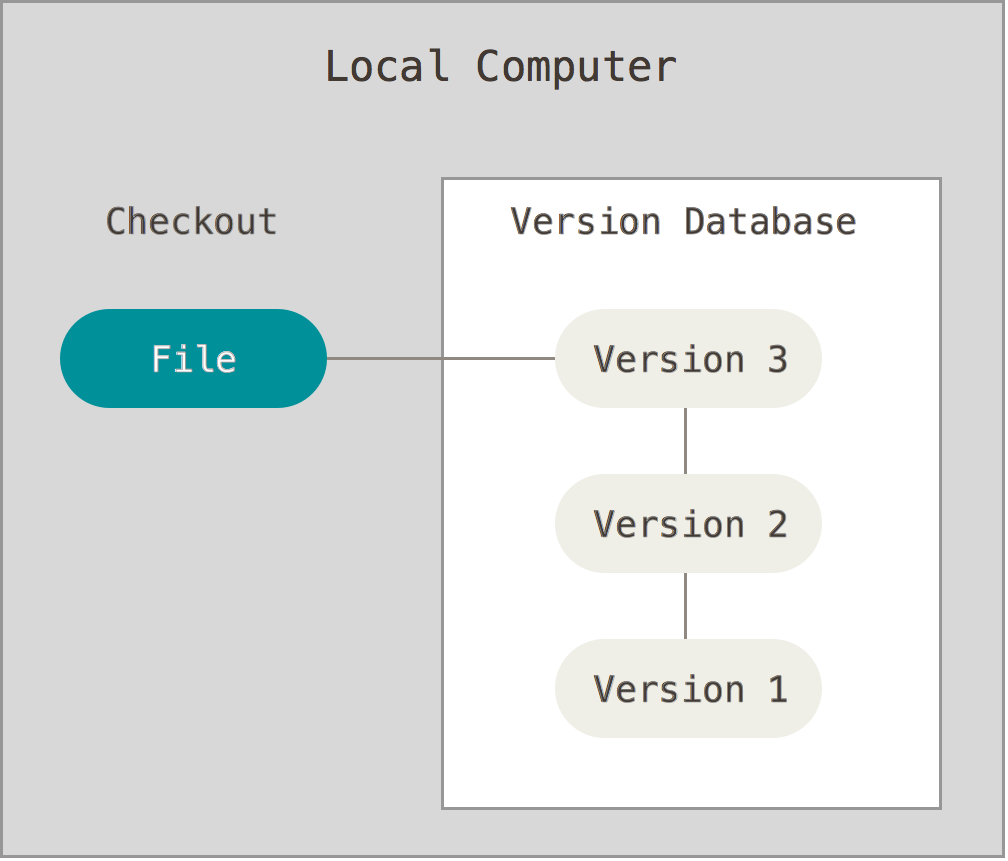
\includegraphics[width=0.5\textwidth]{VersionControlLocal.png}
	\caption{Lokālas \textit{VCS} struktūras princips. (\ref{appfig:VersionControlLocal} pielikumā.)}
	\label{fig:VersionControlLocal}
\end{figure}
Pirmā \textit{VCS} bija \textit{Source Code Control System} (\textit{SCCS}), ko 1972. gadā uzrakstīja \textit{Marc Rochkind}, viens no \textit{Bell Labs} izstrādātājiem. Tā tika radīta \textit{IBM} lieldatoriem (angl. \textit{mainframe}) un bija speciāli paredzēta programmatūrai, kā arī skaidri definēja versiju vēsturi. \textit{SCCS} ieviesa galvenās (angl. \textit{major}) un papildversijas (angl. \textit{minor}) numurēšanu.
Otrā VCS, kas tika radīta, ir \textit{GNU Revision Control System} (\textit{RCS}), un to izmanto arī mūsdienās. \textit{RCS} tika radīta 1980-o gadu sākumā un tā darbojas pēc līdzīga principa kā \textit{SCCS}. \textit{RCS} ir viegla un ar mazu virstēriņu (angl. \textit{low-overhead}), salīdzinot ar vēlākām un spējīgākām \textit{VCS}. \cite{chacon2014progit}

\subsection{Centralizētas \textit{VCS}}
Lokālas \textit{VCS} ir lieliskas, lai atvieglotu viena izstrādātāja darbu, bet ar lokālām \textit{VCS} ir grūti kopīgi strādāt vairākiem cilvēkiem. Lai to atrisinātu, tika radītas centralizētas \textit{VCS} jeb \textit{CVCS}\nomenclature{CVCS}{Centralizēta versiju vadības sistēma (angl. \textit{Centralized Version Control System})}. Šādām sistēmām, piemēram \textit{CVS}, \textit{Subversion} un \textit{Perforce}, ir viens serveris, uz kura atrodas visas datnes un no kura vairāki klienti tās var paņemt. Salīdzinot ar lokālām \textit{VCS}, šādi būtiski uzlabojas spēja sadarboties. Tomēr \textit{CVCS} sistēmām ir arī būtiskas problēmas. Visas datņu versijas atrodas tikai un vienīgi uz servera, bet klientam ir tikai tā versija, kuru tas paņēmis. Tāpēc, ja centrālais serveris atsakās darboties, izstrādātāju darbs praktiski tiek paralizēts, jo nav iespējams paņemt jebkuru versiju vai iesūtīt (angl. \textit{commit}) savas izmaiņas. Ja uz centrālā servera rodas datu bojājumi, ir iespējams pazaudēt visu projekta vēsturi, ja \textit{VCS} datubāze nav dublēta.
\textit{CVCS} atvieglo sadarbību, bet tās centralizētais raksturs pieļauj projekta vēstures zaudēšanu, jo klientam ir tikai tā versija, ko tas paņēmis no centrālā servera. \textit{CVCS} struktūra redzama \ref{fig:VersionControlCentralized} attēlā. \cite{chacon2014progit}
\begin{figure}[H]%!ht
	\centering
	\captionsetup{justification=centering}
	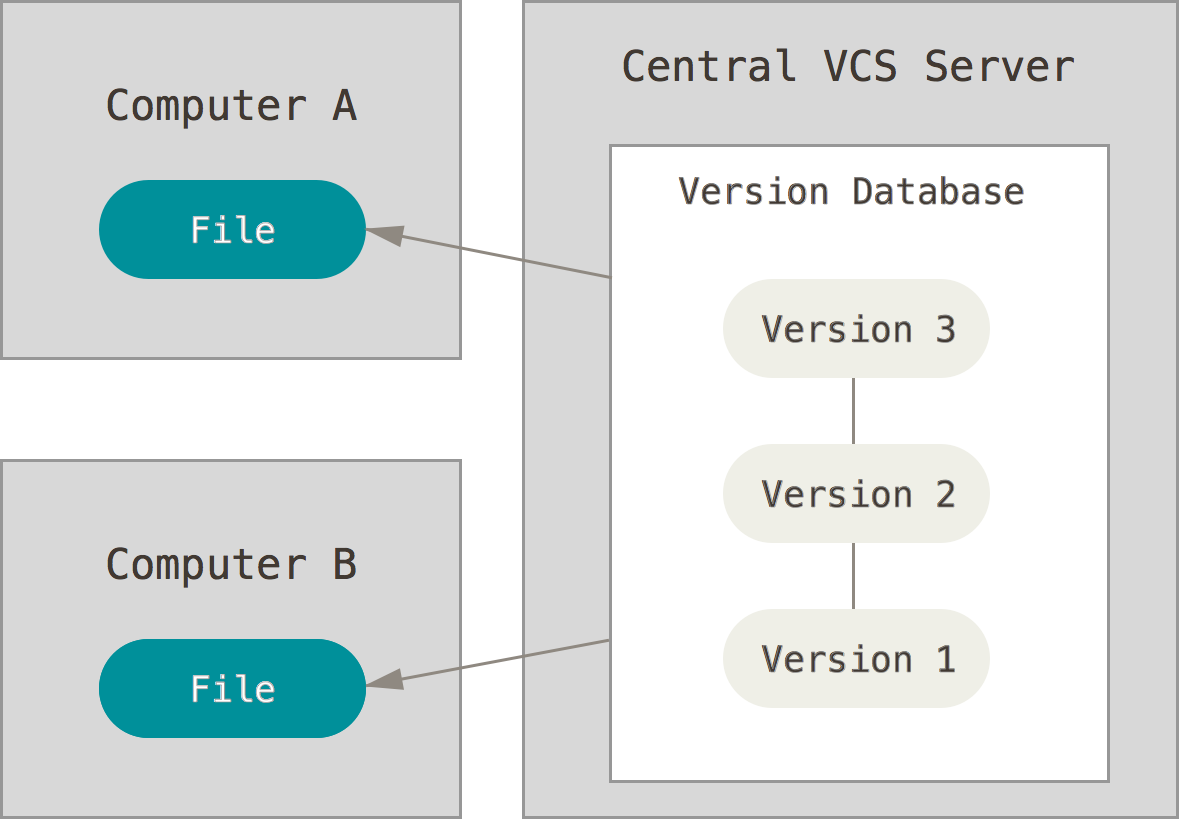
\includegraphics[width=0.5\textwidth]{VersionControlCentralized.png}
	\caption{Centralizētas \textit{VCS} (\ref{appfig:VersionControlCentralized} pielikumā.)}
	\label{fig:VersionControlCentralized}
\end{figure}
Pirmais \textit{CVCS} piemērs ir \textit{Concurrent Version System} (\textit{CVS}). Tā guva popularitāti ap 1990. gadu. Datu saglabāšanai tā izmanto \textit{RCS}, bet \textit{CVS} ieviesa jaunas idejas, lai izstrādātāji varētu sadarboties. Tika ieviests sapludināšanas princips, kā arī centralizēts serveris, uz kura glabājas repozitorijs.
Populārākā un labākā \textit{CVCS} ir \textit{Apache Subversion} (\textit{SVN}). Tās pirmā stabilā versija tika izdota 2004. gadā. SVN izmanto līdzīgu terminoloģiju kā \textit{CVS}, bet tā ir tīrāka. \textit{SVN} ir arī daudz stabilāka un spējīgāka par \textit{CVS}.
\cite{raymondVCS}

\subsection{Dalītas \textit{VCS}}
\textit{CVCS} problēmas atrisina dalītas \textit{VCS} jeb \textit{DVCS}\nomenclature{DVCS}{dalīta versiju vadības sistēma (angl. \textit{Distributed Version Control System})}.\textit{DCVS} sistēmās, kā \textit{Git}, \textit{Mercurial}, \textit{Bazaar}, \textit{Darcs}, joprojām izmanto centralizētu serveri, uz kuru klienti iesūta savas izmaiņas, bet, atšķirībā no \textit{CVCS}, klienti nepaņem tikai datņu pēdējās versijas, bet pilnībā visu projekta vēsturi. Tādējādi, galvenajam serverim atsakoties darboties, projekta vēsturi ir iespējams atjaunot no jebkura klienta. Trešās paudzes \textit{VCS} piemēri ir \textit{GNU Arch}, \textit{Bazaar}, \textit{Monotone}, \textit{BitKeeper} un \textit{Git}. \textit{DVCS} struktūra attēlota \ref{fig:VersionControlDistributed} attēlā. \cite{chacon2014progit}
\begin{figure}[H]%!ht
	\centering
	\captionsetup{justification=centering}
	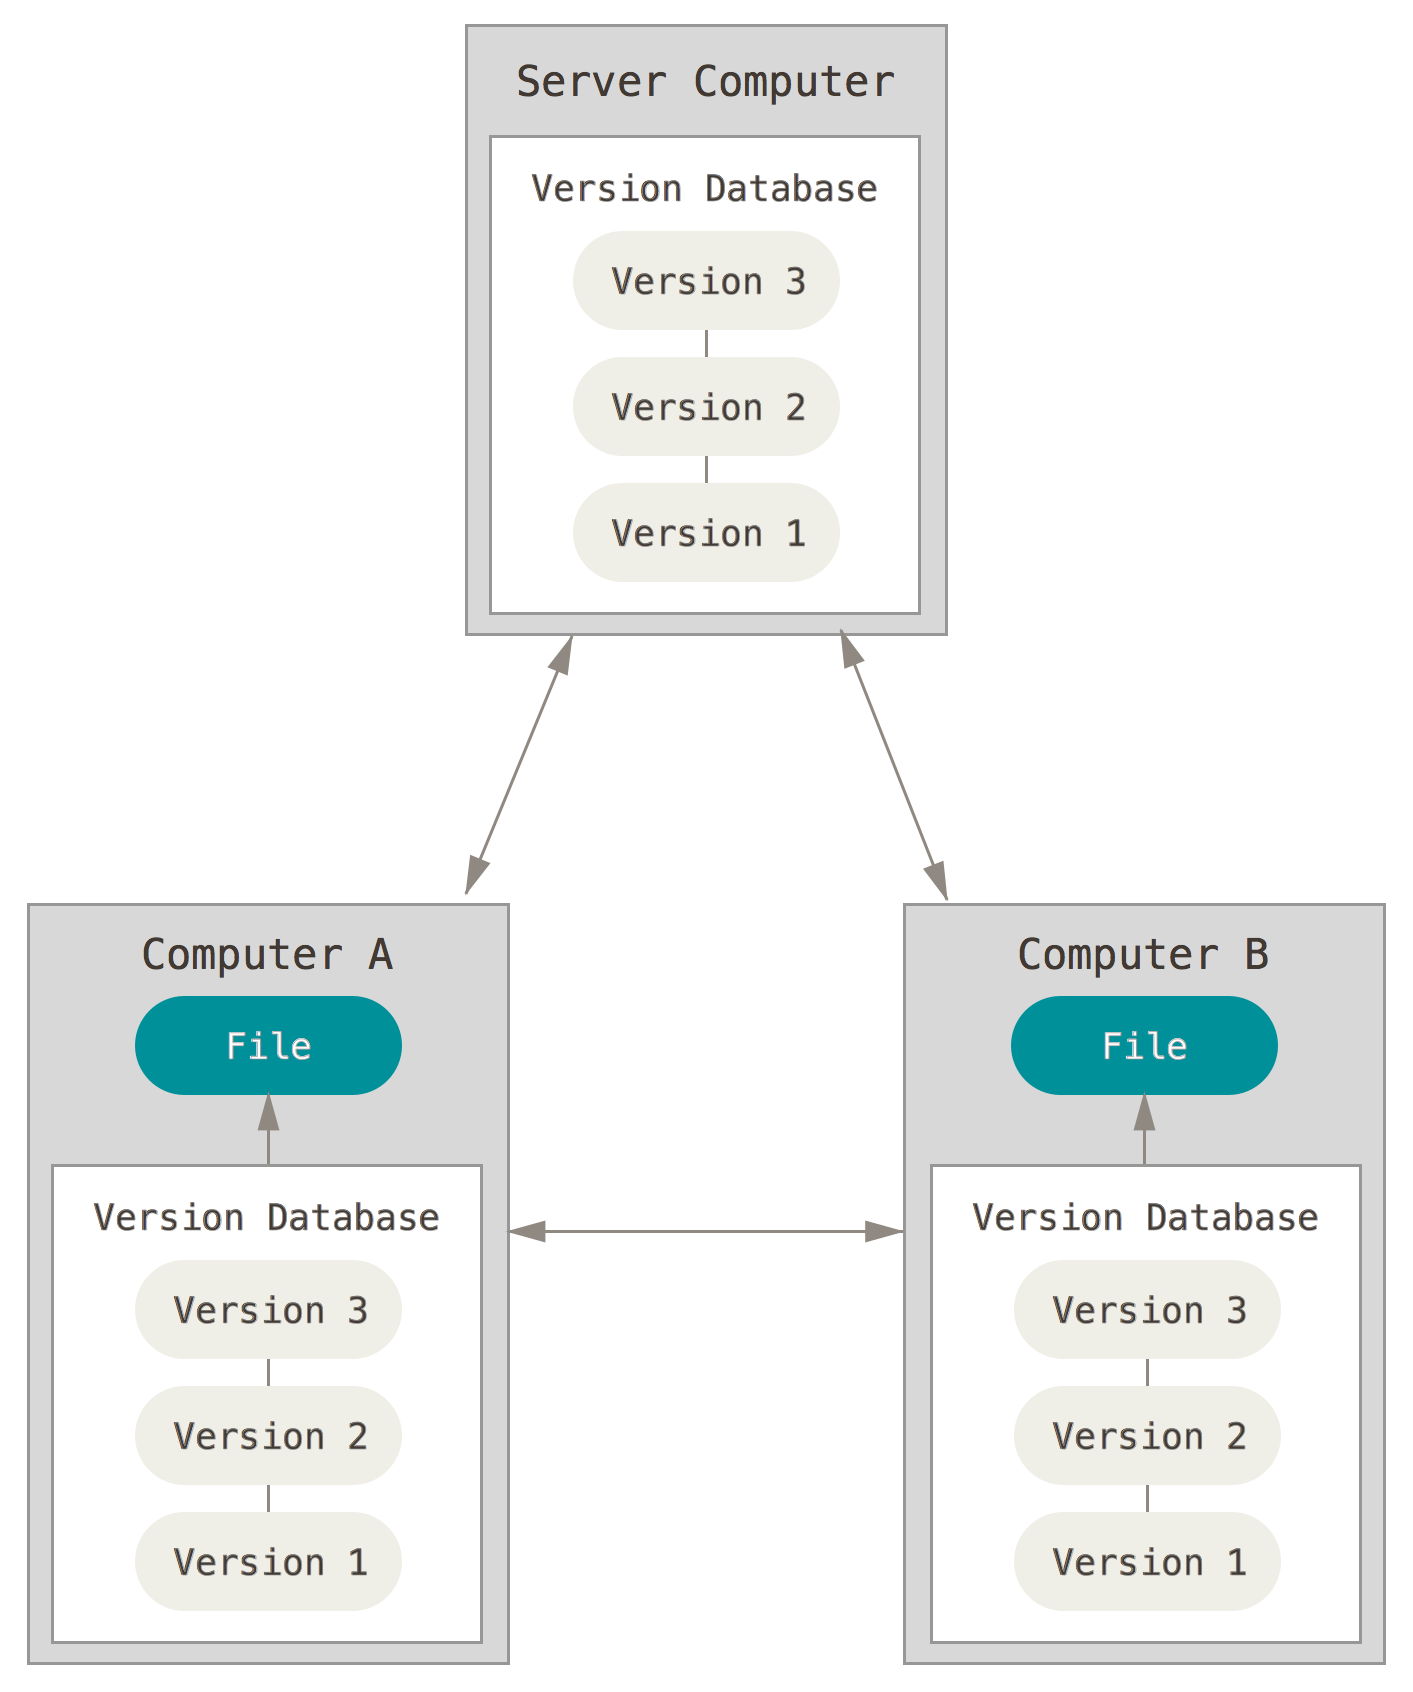
\includegraphics[width=0.5\textwidth]{VersionControlDistributed.png}
	\caption{Dalītas \textit{VCS} (\ref{appfig:VersionControlDistributed} pielikumā.)}
	\label{fig:VersionControlDistributed}
\end{figure}

\section{Versiju vadības sistēma \textit{Git}}
% Kas ir repo?
Darbā tika izmantota \textit{Git} versiju kontrole. % Vēl ko vajag
\textit{Git} ir \textit{DVCS}, ko 2005. gadā radīja Linus Torvals kopā ar \textit{Linux} kodola (angl. \textit{Linux kernel}) izstrādātāju komandu, lai aizvietotu trešās puses \textit{DVCS}  \textit{BitKeeper}, kuras autori \textit{BitMover} 2005. gadā izlēma vairs nepiedāvāt bezmaksas versijas  \textit{Linux} kodola izstrādātājiem. Tāpēc \textit{Linux} kodola izstrādātāji nolēma radīt savu \textit{VCS}, ko izmantot \textit{Linux} kodola versiju vadībai. Galvenie mērķi jaunajai sistēmai bija, lai tā būtu ātra, pilnībā dalīta, spētu būt neatkarīga no galvenā servera, kā arī spētu efektīvi apstrādāt lielus projektus un atbalstītu nelineāru izstrādi, ļaujot vairākiem izstrādātājiem strādāt pie atšķirīgiem uzdevumiem un arī atšķirīgām programmatūras versijām.

\subsection{Kā strādā  \textit{Git}}
 \textit{Git} piedāvā līdzīgu lietotāja saskarni kā citas  \textit{VCS}, bet iekšienē tas datus uztver citādāk. Lielākā daļa  \textit{VCS} saglabā veikto izmaiņu sarakstu kā datnes un to izmaiņas jeb deltas.
% Attēls https://git-scm.com/book/en/v2/Getting-Started-Git-Basics
Turpretī  \textit{Git} katru versiju uztver kā failu sistēmas momentuzņēmumu. Katra saglabātā versija saglabā esošo projekta stāvokli, un, lai sistēma būtu efektīvāka, uz datnēm, kuras nav mainītas,  \textit{Git} izveido atsauces.  \textit{Git}, uztverot versijas kā failu sistēmas momentuzņēmumus, atļauj ļoti efektīvi veidot nelineāras darbplūsmas (angl. \textit{Workflow}).
% Attēls un arī varētu piemēru no Pluralsight video.
Vēl viens būtisks ieguvums no  \textit{DVCS} ir tas, ka lielāko daļa darbību ir iespējams izdarīt lokāli, bezsaistē. Tas nozīmē, ka  \textit{Git} ir ļoti ātrs, jo lielākajai daļai darbību nav nekāda tīkla virstēriņa, kas ir tipisks mīnuss \textit{CVCS}.
% Nearly every operation is local

Pirms \textit{Git} saglabā datus, lai nodrošinātu datu integritāti, tas visam izveido \textit{SHA-1} kontrolsummu (angl. \textit{Checksum}) un pēc tam veido atsauces, izmantojot izveidotās kontrolsummas. Savā datubāzē \textit{Git} saglabā visu pēc datņu satura kontrolsummas, nevis pēc to nosaukuma. Tas nozīmē, ka ir neiespējami izdarīt izmaiņas tā, lai \textit{Git} par tām nezinātu. Tā Git spēj atklāt datu bojājumus, kas radušies tīkla vai cietā diska bojājumu gadījumā. Kā arī, gandrīz visas \textit{Git} darbības pievieno datus datubāzē, tāpēc bieži ir iespējams atgūt datus, kuri šķiet neatgriezeniski pazaudēti.

Strādājot ar \textit{Git}, jāņem vērā, ka faili var atrasties kādā no trīs stāvokļiem. Fails var būt iesūtīts, izmainīts vai sagatavots (angl. \textit{staged}). Darba direktorijs satur kādu konkrētu versiju, pie kuras tiek strādāts. Sagatavošanas stāvoklis atļauj pievienot failus, pie kuriem tiek strādāts, savam iesūtījumam, tādējādi iespējams iekļaut tikai daļu no savām izmaiņām. Jāņem vērā, ka izmaiņas, kuras tiks veiktas pēc failu sagatavošanas, netiks ņemtas vērā, ja arī tās nesagatavos iesūtījumam. Sagatavotos failus iespējams iesūtīt \textit{Git} direktorijā, kurā tie tiks saglabāti objektu datubāzē.
Trīs \textit{Git} stāvokļi redzami attēlā \ref{fig:Git3Areas}. \cite{chacon2014progit}
\begin{figure}[H]%!ht
	\centering
	\captionsetup{justification=centering}
	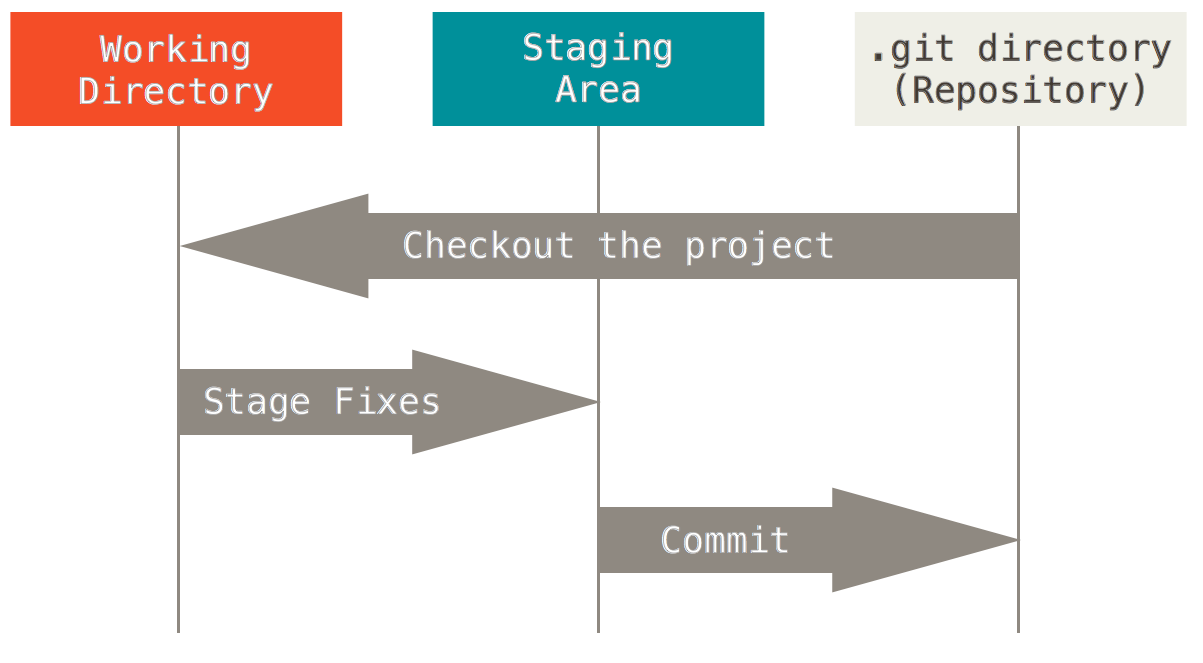
\includegraphics[width=0.5\textwidth]{Git3Areas.png}
	\caption{\textit{Git} stāvokļi}
	\label{fig:Git3Areas}
\end{figure}

\subsection{Zarošanās} \label{Branching}
\textit{Git} zarošanās (angl. \textit{Branching}) ir ļoti spējīgs mehānisms, kas ļauj veikt eksperimentus, nemaz netraucējot jau uzrakstītajam kodam. Turklāt \textit{Git} ir spējīgs izveidot zaru ļoti ātri, jo dalītais sistēmas raksturs nodrošina, ka viss repozitorijs ir pieejams arī lokāli. Tādējādi iespējams jebkuru izveidoto iesūtījumu ņemt kā pamatu jaunam zaram, uz kura veikt izstrādi. Izmantojot zarošanos, ir iespējams vienlaicīgi uzturēt pat vairākas programmatūras versijas, piemēram, veicot drošības labojumus novecojušai versijai, lai netraucētu jaunās versijas izstrādei.
\subsubsection{Izvēlētā zarošanās stratēģija}
% http://nvie.com/posts/a-successful-git-branching-model/
% https://www.atlassian.com/git/tutorials/comparing-workflows/gitflow-workflow
Darbā izvēlēts izmantot  \textit{Gitflow} darbplūsmu, kas ir īpaši lietderīga lieliem projektiem, jo Gitflow darbplūsma skaidri nosaka repozitorija zaru funkcijas.  \textit{Gitflow} pamatā galvenie ir divi zari: pamatzars (angl. \textit{master}) un izstrādes zars (angl. \textit{develop}). Pamatzars atspoguļo relīžu vēsturi, un koda iesūtījumi ir atzīmēti ar versiju numuriem. Katru reizi, kad pamatzarā tiek veikta kāda izmaiņa, to atzīmē ar jaunu versijas numuru. Izstrādes zars kalpo pievienotās funkcionalitātes integrācijai. Tomēr katrai pievienotajai iespējai vajadzētu atrasties savā funkcionalitātes (angl. \textit{feature}) zarā. Citās darbplūsmās parasti atzarojas no pamatzara, bet  \textit{Gitflow} darbplūsmā atzarošanās tiek veikta no izstrādes zara. Katra jaunā iespēja atzarojas no izstrādes zara, un, kad tā ir pabeigta, tā tiek sapludināta ar izstrādes zaru.
Kad pienāk laiks jaunai relīzei, no izstrādes zara atzarojas relīzes zars. Relīžu zaros nekad netiek pievienota jauna funkcionalitāte. Relīzes zari tiek  izmantoti tikai tālākai koda sagatavošanai nākamajai versijai, tajā veic tikai labojumus. Tajā nepievieno papildus funkcionalitāti. Kad relīze ir gatava, to sapludina ar pamatzaru, atzīmē ar jaunu versijas numuru un sapludina arī ar izstrādes zaru.
Apkopes (angl. \textit{maintenance}) zari tiek izmantoti, lai ātri veiktu labojumus relīzēm. Apkopes zars atzarojas no pamatzara un, tiklīdz labojums ir pabeigts, tas tiek sapludināts ar pamatzaru un izstrādes zaru, vai vēl neizlaistu relīzes zaru.

Šāda vairākzaru darbplūsma ļauj izstrādei neapstāties pie viena uzdevuma, piemēram, nespiež strādāt tikai pie relīzes vai papildu funkcionalitātes izstrādes. Tā kā ir vairāki zari gan relīzēm, gan funkctionalitātei, komandas var strādāt paralēli, katra pie sava uzdevuma, nebojājot repozitoriju citām komandām.
 \textit{Gitflow} darbplūsma redzama attēlā \ref{fig:WorkflowGitflow}. Šīs un citu darbplūsmu piemēri atrodami resursā \cite{workflow-comparison}.
\begin{figure}[H]%!ht
	\centering
	\captionsetup{justification=centering}
	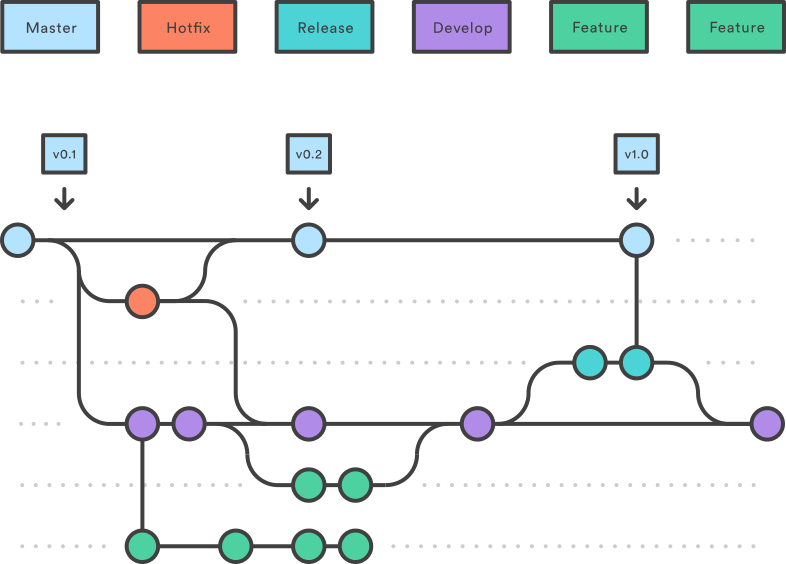
\includegraphics[width=0.5\textwidth]{WorkflowGitflow.png}
	\caption{\textit{Gitflow} zarošanās stratēģijas attēlojums (\ref{appfig:WorkflowGitflow} pielikumā.)}
	\label{fig:WorkflowGitflow}
\end{figure}
Pamatzars atspoguļo mājaslapas kodu, kas strādās uz \textit{RaspberryPi} tīkla servera. Tiklīdz kā tiks atjaunināts pamatzars, serveris to lejupielādēs un sāks izmantot jaunāko koda relīzi.
Izstrādes zars izmantots izmaiņu integrēšanai.
Galvenais darbs notiks uz funkcionalitātes zariem, kuros fokusēti tiks nodalīta laika gaitā pievienotā funkcionalitāte.



Darba praktiskā daļa ir sadalīta divos repozitorijos. Viens repozitorijs -- piekļuves sistēmas administrēšanas mājaslapai, otrs -- infrastruktūras uzstādīšanai ar \textit{Chef}.

\chapter{Konfigurācijas pārvaldība}
Šajā nodaļā apskatīta konfigurācijas pārvaldības nozīmība un īstenošana, izmantojot konfigurācijas pārvaldības rīku \textit{Chef}, kas ļauj aprakstīt infrastruktūru kodā.
Konfigurācijas pārvaldība nodrošina vispārēju sistēmas vadību un satur datus no pārvaldāmajiem objektiem. Sākot ar 1960-ajiem gadiem, konfigurācijas datus saglabā datu bāzē, ko konfigurācijas pārvaldnieks var izmantot iekārtu (darbstaciju, serveru, maršrutētāju, u.c.) konfigurēšanai.
Konfigurācijas pārvaldība palīdz nodrošināt komponenšu un sistēmas kvalitāti, to atbilstību noteiktajajām tehniskajām prasībām, kā arī palīdz veikt sistēmu auditēšanu.

\section{Infrastruktūra kā kods}
Sistēmas administratori vienmēr centušies automatizēt sistēmu uzstādīšanu un konfigurēšanu. Ierasts izmantot \textit{bash} skriptus, kuros secīgi sarakstītas izpildāmās komandas konfigurācijas veikšanai. Ar laiku tika radīta specializēta programmatūra, kas ļauj infrastruktūru aprakstīt kodā un automatizēt sistēmu uzstādīšanu un konfigurēšanu. Pašlaik populārākie rīki ir 2005. gadā radītais \textit{Puppet}, 2009. gadā radītais \textit{Chef} un 2012. gadā radītais \textit{Ansible}. Šie rīki ļauj visu infrasturktūru aprakstīt kodā -- sistēmu konfigurāciju, ieskaitot lietotāju pārvaldību. Darbā izmantots konfigurācijas pārvaldības rīks \textit{Chef}, kas ir uzrakstīts, izmantojot \textit{Ruby} un \textit{Erlang} programmēšanas valodas.

\textit{Chef} ir spēcīga automatizēšanas platforma, kas apraksta sarežģītu infrastruktūru kodā, neatkarīgi no tā, vai resursi atrodas mākonī\nomenclature{Mākonis}{Mākoņdatošana (angl. \textit{Cloud computing})}, uz lokāliem serveriem vai to kombinācijā. \textit{Chef} spēj automatizēt kā lietotnes ir konfigurētas, izvietotas un pārvaldītas, neatkarīgi no uzstādītās infrastruktūras izmēra.

\textit{Chef} pamatā ir vienkārša koncepcija: vēlamā stāvokļa sasniegšana, centralizētas IT infrastruktūras modelēšana un resursu primitīvi, kas kalpo kā platformas pamatelementi. Šī koncepcija ir tas, kas rīkam ļauj efektīvi pārvaldīt pat ļoti sarežģītas infrastruktūras. \cite{chef-docs}
% Automatizēta, abstahēta, vienkāršota
\subsection{Chef komponentes}
Konfigurācijas orķestrēšanai \textit{Chef} strādā pēc vedējsekotājsistēmas (angl. \textit{Master-slave system}) principa. Galvenais ir \textit{Chef} serveris, kurš pārvalda infrastruktūru.
Diagrammā \ref{fig:ChefOverview} redzamas \textit{Chef} komponenšu attiecības starp \textit{Chef} serveri, mezgliem (angl. \textit{nodes}) un izstrādātāja darbstaciju. \cite{chef-docs}
\begin{figure}[H]%!ht
	\centering
	\captionsetup{justification=centering}
	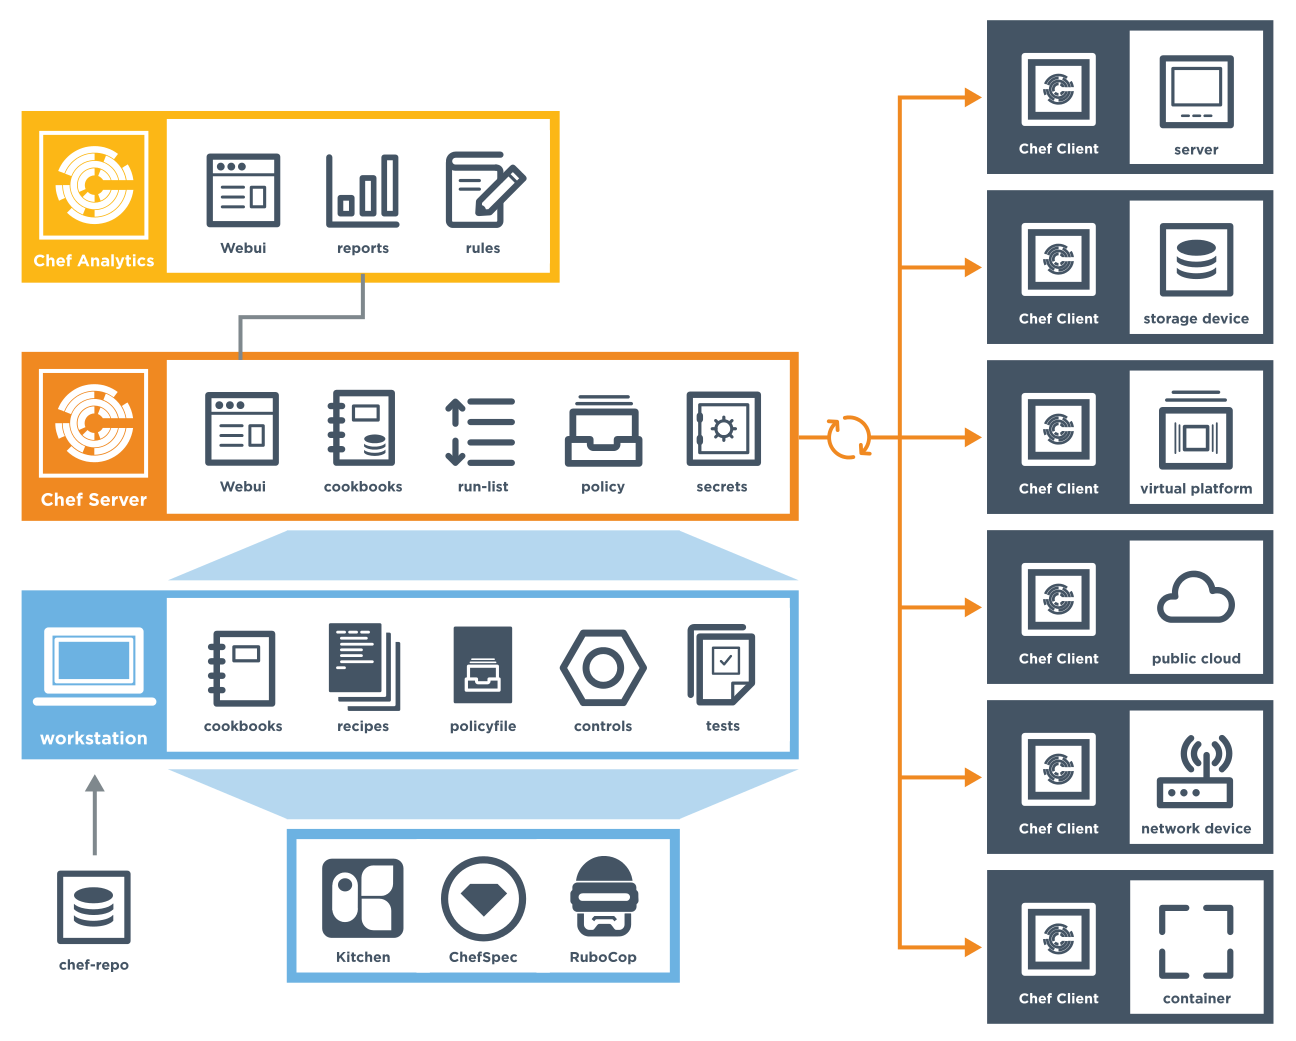
\includegraphics[width=0.5\textwidth]{ChefOverview.png}
	\caption{Chef komponentes (\ref{appfig:ChefOverview} pielikumā.)}
	\label{fig:ChefOverview}
\end{figure}
Galvenās \textit{Chef} komponentes:
\begin{itemize}
	\item Izstrādātāja darbstacija, kas ir konfigurēta darbam ar \textit{Chef} platformu. Vissvarīgākais nepieciešamais, lai sāktu izstrādi ar \textit{Chef}, ir lai darbstacijā būtu uzinstalēta \textit{Ruby} programmēšanas valoda, bet ieteicams izmantot ne tikai to, bet arī \textit{Chef} izstrādes rīkkopu (angl. \textit{Chef development kit}), kas satur arī citas izvēles pakotnes, ieskaitot \textit{Chef} komandrindas rīku, \textit{Kitchen}, \textit{ChefSpec}, \textit{Berkshelf}, u.c. rīkus.
	\item \textit{Chef}, lai aprakstītu lielu daļu konfigurācijas, izmanto domēnam specifisku valodu, kas balstīta uz \textit{Ruby} programmēšanas valodu un izmanto tās sintaksi. \textit{Chef} ir ļoti pielāgojams, jo ļauj pilnībā izmantot \textit{Ruby} valodas dotās iespējas.
	\item Mezgli ir jebkuras sistēmas (fiziskas, virtuālas, mākonis, u.t.t.), kuras pārvalda ar \textit{Chef} platformu. \textit{Chef} klients (angl. \textit{chef-client}) ir izpildāma programma, kas uzstādīta uz katra mezgla. Šis klients izpilda visus konfigurācijas uzdevumus.
	\item \textit{Chef} serveris kalpo kā centrmezgls. Konfigurācija tiek augšupielādēta uz \textit{Chef} servera no darbstacijām. \textit{Chef} klients savienojas ar \textit{Chef} serveri un saņem tā konfigurācijas datus.
	\textit{Chef} pārvaldības konsole ir \textit{Chef} servera lietotāja saskarne, ko lieto, lai pārvaldītu datu pakas (satur privātus konfigurācijas datus, kurus iespējams šifrēt), rekvizītus, izpildāmās receptes (angl. \textit{run_list}), lomas, vidi, recepšu grāmatas.
	\item \textit{Chef} analīze - satur informāciju par to, kas notiek uz \textit{Chef} servera, ieskaitot veiktās izmaiņas, izmaiņu autoru un veikto izmaiņu laiku. Šo informāciju nosūta \textit{Chef} klienta izpildprogramma, kad tā pabeigusi savu darbu. Tādējādi iespējams sistēmu auditēt.
	\item \textit{Chef} lielveikals (angl. \textit{Chef Supermarket}) -- šeit atrodas brīvi izmantojamas \textit{Chef} kopienas recepšu grāmatas. Tajā jau ir gandrīz trīs tūkstoši sagatavotu recepšu grāmatu, kuras spēj veikt lielāko daļu konfigurācijas daudziem rīkiem.
\end{itemize}



\textit{Chef} platformas pamatā galvenais ir \textit{Chef} repozitorijs, kurā glabājas viss konfigurācijas kods. Izstrādātājs lejupielādē repozitoriju uz lokālās darbstacijas un uz tās veic arī turpmāko izstrādi. Repozitorijā atrodas recepšu grāmatas (angl. \textit{cookbooks}), kurās atrodas receptes (angl. \textit{recipes}).
Izmantojot \textit{Chef} izstrādes rīkkopu, izstrādātājs uz savas darbstacijas var rakstīt konfigurāciju.
Uzrakstīto kodu ir iespējams arī testēt. Ir iespējams pārbaudīt uzģenerēto datņu, izpildīto komandu atbilstību vēlamajam ar vienību testiem (angl. \textit{unit test}) izmantojot \textit{ChefSpec}, kā arī testēt ar integrācijas testiem (angl. \textit{integration test}), izmantojot testu virtuvi (angl. \textit{Test Kitchen} \url{http://kitchen.ci/}). Integrācijas testi ļauj pārbaudīt, kā viss strādā kopā, jo testu virtuve izveido jaunu sistēmas eksemplāru mākonī vai uz lokālās darbstacijas, izmantojot \textit{Vagrant} virtuālās mašīnas vai \textit{Docker} konteinerus. Ir izveidotas arī koda kvalitātes un stila pārbaudes, ko iesaka izmantot vismaz kopienas recepšu grāmatās, tādējādi cenšoties kopienas recepšu grāmatas padarīt konsistentākas.
Izmantojot \textit{Chef}izstrādes rīkkopas rīku \textit{knife}, izstrādātājs lielāko daļu darba var veikt no lokālās darbstacijas. \textit{Knife} ļauj augšuielādēt recepšu grāmatas uz \textit{Chef} servera, pārvaldīt uzstādītos mezglus, kā arī pievienot jaunus mezglus \textit{Chef} serverim.

\textit{Chef} platforma strādā pēc vedējsekotājsistēmas principa, kas nozīmē, ka vienmēr ir \textit{Chef} serveris, kas kalpo kā centrmezgls un pārvalda visus uzstādītos mezglus. Atkarībā no uzņēmuma vajadzībām, \textit{Chef} serveri ir iespējams uzstādīt vairākos veidos. \textit{Chef} platforma piedāvā \textit{Chef} serveri kā pakalpojumu (\textit{Hosted Chef}), kuru ir iespējams izmantot par brīvu līdz 5 mezgliem. Šis ir vienkāršākais un ātrākais veids, kā praktiski sākt strādāt ar \textit{Chef} platformu, tomēr uzņēmumiem tas varētu būt neatbilstošs, jo nav pilnīga kontrole pār serveri. Ir iespējams \textit{Chef} serveri uzstādīt mākonī. Ir pieejami jau gatavi instanču attēli \textit{Amazon Webservices} un \textit{Microsoft Azure} mākoņos, kas būtiski paātrina \textit{Chef} servera uzstādīšanas laiku. Kā arī \textit{Chef} serveri ir iespējams uzstādīt uz jebkura servera, uz kura uzstādīta \textit{Red Hat Enterprise Linux} vai \textit{CentOS} 5., 6. vai 7. versija, vai Ubuntu 10.04, 12.04 vai 14.04 versija.
Tā kā darbā uzstādīta tikai viena servera instance, izmantojot \textit{Chef}, darbā izmantots \textit{Hosted Chef} serviss. Tā arī ir paredzēts un ieteicams izmantot \textit{Chef} platformu. Apskatīts arī, kā izmantot \textit{Chef} rīka piedāvātās automatizācijas iespējas bez \textit{Chef} servera instances, tomēr nevar teikt, ka tas ir ieteicams variants.

\subsection{Izstrādātāja darbstacijas sagatavošana darbam ar \textit{Chef}} \label{ChefDarbstacija}
Veigsmīgam darbam ar \textit{Chef} ir ieteicams uz darbstacijas uzstādīt šādu programmatūru:
\begin{itemize}
	\item \textit{ChefDK} (\url{https://downloads.chef.io/chef-dk/})
	\item \textit{VirtualBox} (\url{https://www.virtualbox.org/})
  \item \textit{Vagrant} (\url{https://www.vagrantup.com/})
  \item Teksta redaktors
\end{itemize}
Lai sāktu lietot \textit{Chef}, ir nepieciešams uz darbstacijas uzstādīt vismaz \textit{chefDK}. \textit{chefDK} sevī ietver \textit{Ruby} programmēšanas valodas izpildāmos failus, kā arī bibliotēkas darbam ar \textit{Chef}.
\textit{VirtualBox} un \textit{Vagrant} uzstādīšana nav obligāta, bet ieteicama, lai veiktu integrācijas testus uz darbstacijas, izmantojot \textit{KitchenCI} (\url{http://kitchen.ci/}).
% Ir galvenais Chef serveris uz kura glabājas vairākas komponentes:
% \begin{itemize}
% 	\item recepšu grāmatas (angl. \textit{cookbooks}) - kurās atrodas receptes (angl. \textit{recipes}).
% \end{itemize}
% Chef struktūra
% Chef repozitorijs - nosaka konfigurācijas pārvaldības struktūru. Repozitorijs satur:
% 	Recepšu grāmatas\nomenclature{Cookbooks}{Recepšu grāmatas (angl. \textit{cookbooks}) - satur receptes}
% 		Receptes\nomenclature{Recipes}{Receptes (angl. \textit{recipes}) - tajās konfigurācija tiek aprakstīta kodā.}
% 		Rekvizīti\nomenclature{Attributes}{Rekvizīti (angl. \textit{attributes}) - tie var tikt definēti recepšu grāmatā vai receptē un tos var izmantot, lai pārlabotu noklusējuma iestatījumas uz mezgla.}
% 	Datu somas\nomenclature{Data bags}{Datu somas (angl. \textit{data bags}) - līdzīgi rekvizītiem, tās izmanto noklusēto iestatījumu pārlabošanai. Atšķirībā no rekvizītiem, datu somas ir iespējams šifrēt.}
% 	Vide\nomenclature{Environment}{Vide (angl. \textit{environment}) - katram mezglam ir noteikta vide, ar kuru iespējams noteikt izmantoto recepšu versijas.}
% 	Lomas\nomenclature{Roles}{Lomas (angl. \textit{roles}) }
%
% Chef serveris
% 	Nodes
% 		Chef-client
% 		Run-list
% 			Cookbooks
% 		Attributes
% 		Environment

% Chef struktūra
% \begin{itemize}
% 	\item Chef repozitorijs
% 	\begin{itemize}
% 		\item Cookbooks
% 		\begin{itemize}
% 			\item Recipes
% 			\item Attributes
% 		\end{itemize}
% 		\item Data_bags
% 		\item Environments
% 		\item Roles
% 	\end{itemize}
% 	\item Chef-server
% 	\begin{itemize}
% 		\item Chef repozitorijs
% 		\item Nodes
% 		\begin{itemize}
% 			\item Chef-client
% 			\item Run-list
% 			\item Cookbooks
% 			\item Attributes
% 			\item Environment
% 		\end{itemize}
% 	\end{itemize}
% \end{itemize}

\chapter{\textit{Ruby on Rails}}
% Darbā tika radīta mājaslapa telpas piekļuves administrēšanai izmantojot Ruby on Rails satvaru.
\textit{Rails} ir tīmekļa lietojumprogrammu jeb aplikāciju satvars (angl. \textit{web application framework}), kas radīts, izmantojot \textit{Ruby} programmēšanas valodu. Deivids Heinemers Hansons (angl. \textit{David Heinemeier Hansson}) radīja un izdeva pirmo \textit{Rails} versiju 2004. gadā kā atvērtā koda programmatūru. Kopš izdošanas brīža \textit{Rails} ir kļuvis par vienu no spējīgākajiem un populārākajiem dinamisku mājaslapu izstrādes rīkiem. \textit{Rails} kļuvis populārs, jo praktiski ir izveidota domēnam specifiska valoda jeb \textit{DSL} \nomenclature{DSL}{Domēnam specifiska valoda (angl. \textit{Domain specific language})} mājaslapu izstrādei. Tādējādi daudzi bieži sastopami izstrādes uzdevumi, piemēram, \textit{HTML} \nomenclature{HTML}{Hiperteksta iezīmēšanas valoda (angl. \textit{HyperText Markup Language})} ģenerēšana, datu modeļu veidošana, \textit{URL} \nomenclature{URL}{Vienotais resursu vietrādis (angl. \textit{Uniform Resource Locator})} maršrutēšana ir viegli veicama, izmantojot \textit{Rails}, un galu galā izveidotais aplikācijas kods ir saprotams un viegli lasāms. \textit{Rails} arī mēdz ātri pielāgoties tīmekļa tehnoloģiju jaunumiem. Piemēram, \textit{Rails} bija viens no pirmajiem satvariem, kas ieviesa \textit{REST} \nomenclature{REST}{Reprezentācijas stāvokļa pārsūtīšana (angl. \textit{Representational state transfer})} arhitektūras stilu tīmekļa aplikācijās.

\textit{Rails} ir radīts, lai padarītu dinamisku mājaslapu izveidi vieglāku un ātrāku, veicot vajadzīgus pieņēmumus, lai izstrādātājs varētu uzreiz sākt strādāt. Izmantojot \textit{Rails} satvaru, uzrakstot nedaudz koda, var panākt daudz vairāk nekā izmantojot citas programmēšanas valodas vai tīmekļa lietojumprogrammu satvarus. \textit{Rails} doktrīnā viens no punktiem ir "Konvencija pāri konfigurācijai" (angl. \textit{Convention over configuration}), tas nozīmē, ka \textit{Rails} izstrādātājiem ir atvieglota lēmumu pieņemšana tīmekļa lietojumprogrammu programmēšanā, jo pēc noklusējuma jau ir ielikts pamats, kurā jāmaina tikai specifiskas lietas. Daudzas lietas ir abstrahētas, kas būtiski vienkāršo izstrādi, kā arī \textit{Rails} apgūšanu. Tāpat viens no galvenajiem darbības principiem, ko paturēt prātā, rakstot kodu, ir "Neatkārtot sevi" (angl \textit{Don't repeat yourself}). Tas ir arī labs princips neatkarīgi no programmēšanas valodas, jo tas padara kodu vieglāk uzturamu un saprotamu.
\cite{hartlRails} \cite{rails-guides}

\textit{Rails} sevī ietver visu nepieciešamo, lai radītu ar datubāzi nodrošinātu lietojumprogrammu, kas balstīta uz Modeļa-Skata-Kontroliera \nomenclature{MVC}{Modelis-Skats-Kontrolieris (angl. \textit{Model-View-Controller})} modeļa.
% MVC struktūra ļauj sakārtot kodu un labāk saprast mājaslapas darbību.
\textit{MVC} sadala lietojumprogrammu trīs slāņos, kur katram slānim ir savs pienākums.
Skata slānis satur šablonus, kurus izmanto, lai sagatavotu mājaslapas izskatu un attēlotu ievadītos datus. \textit{Ruby on Rails} izmanto \textit{HTML} šablonus ar integrētu \textit{Ruby} kodu.
Modelis attēlo domēna modeli (piemēram, Lietotāji, Produkti). Būtībā lielākā daļa modeļu ir balstīti uz datubāzi un attēlo tās īpašības.
Kontrolieris apstrādā ienākošos \textit{HTTP} pieprasījumus un dod atbilstošu atbildi. Kontrolieris saņem lietotāja klikšķus, nosūta komandas modelim un galu galā uzģenerē skatus, izmantojot iepriekš izveidotos šablonus.
\cite{rails-api}
\textit{Rails} parūpējas par daudz lietām, kas mēdz radīt kļūdas, piemēram \textit{Rails} veic \textit{SQL} vaicājumu ģenerēšanu. Izstrādātājam nav jāuztraucas par piekļuvi datubāzei, datu ierakstīšanu un to iegūšanu no datubāzes.

\section{Izstrādātāja darbstacijas sagatavošana darbam ar \textit{Ruby on Rails}} \label{RubyDarbstacija}
Lai veiksmīgi sāktu mājaslapas izstrādi, ir nepieciešams sagatavot izstrādes darbstaciju un uzstādīt nepieciešamās pakotnes. Sagatavojot darbstaciju darbam ar \textit{Chef} platformu, kas apskatīta \ref{ChefDarbstacija} nodaļā, \textit{ChefDK} uzstāda tajā iegultus \textit{Ruby} programmēšanas valodas izpildfailus, kurus iespējams arī izmantot \textit{Rails} izstrādei. Tomēr ieteicams izmantot atsevišķu \textit{Ruby} instalāciju. Vienkāršākais veids, kā sagatavot darbstaciju, ir sekot \textit{GoRails} pamācībai: \url{https://gorails.com/setup/ubuntu/14.04}. Darba izstrāde tika veikta uz \textit{Ubuntu} 14.04 operētājsistēmas.


\chapter{Programmatūras izstrādes modeļi}
Ir daudzi modeļi, pēc kuriem var vadīties, izstrādājot programmatūru. Turpmāk tiks apskatīts tradicionālais Ūdenskrituma modelis (angl. \textit{Waterfall model}) un Spējās programmatūras izstrādes modelis (turpmāk \textit{Agile}) \nomenclature{Agile}{Spējā programmatūras izstrāde (angl. \textit{Agile software development})} un novērtēta šo modeļu atbilstība programmatūras izstrādei.
\section{Ūdenskrituma modelis}
Senākais izmantotais modelis, kas aizņemts no ražošanas un būvniecības nozarēm, ir Ūdenskrituma modelis. Šajā modelī ir stingri noteiktas fāzes, kurām sekot izstrādes procesā.
Ūdenskrituma modeļa fāzes ir sekojošas:
\begin{itemize}
	\item sistēmas un programmatūras vajadzības;
	\item analīze, rezultātā iegūstot modeļus un shēmas;
	\item noformēšana, rezultātā iegūstot programmatūras arhitektūru;
	\item programmēšana;
	\item testēšana;
	\item sistēmas uzstādīšana, uzturēšana un atbalstīšana.
\end{itemize}
Ūdenskrituma modelī katrā fāzē veiktais darbs ir galējs. Iepriekšējā fāzē izmaiņas netiek veiktas pēc tās beigām, vismaz ne bez būtiskiem laika un līdzekļu zaudējumiem.
Ūdenskrituma modelis ir aizgūts no būvniecības, un tas ir piemērots, piemēram, tiltu būvniecībā, bet tas ir nebūtisks mūsdienu programmatūras izstrādē, jo nav iteratīvs un katra fāze aizņem daudz laika.


\section{Spējā programmatūras izstrāde}
\textit{Agile} būtībā izpilda tos pašus Ūdenskrituma modeļa soļus, bet krasi atšķirīgā veidā. Ūdenskrituma modelī nav pieļaujama darba sākšana pie nākamās fāzes, kamēr iepriekšējā nav pilnībā pabeigta, turpretī \textit{Agile} spēj ātri adaptēties un veikt pat vairākas iterācijas dienā. Tas nozīmē, ka\textit{ Agile} modelis pieļauj vairākas strādājošas programmatūras relīzes dienā.
\textit{Agile} manifestā ir noteiktas četras vienkāršas vērtības, pēc kurām vadoties var labāk izstrādāt programmatūru:
\begin{itemize}
	\item cilvēki un mijiedarbība pāri procesiem un rīkiem;
	\item strādājoša programmatūra pāri izsmeļošai dokumentācijai;
	\item sadarbība ar klientu pāri līguma sarunām;
	\item spēja reagēt izmaiņām pāri sekošanai plānam.
\end{itemize}
Ar \textit{Agile} var radīt maksimāli daudz vērtības klientiem un citām ieinteresētajām pusēm, piegādājot strādājošu programmatūru pēc iespējas ātrāk un laika gaitā to uzlabojot. To panāk, veicot tikai tik daudz plānošanas, cik nepieciešams, lai sāktu darbu.
\textit{Agile} seko šādiem principiem:
\begin{itemize}
	\item galvenā prioritāte ir pastāvīgi klientam piegādāt un uzlabot vērtīgu programmatūru;
	\item pieņemt mainīgas prasības, pat vēlās izstrādes stadijās;
	\item bieži veikt strādājošas aplikācijas relīzes;
	\item ieinteresētajām pusēm un izstrādātājiem ir pastāvīgi jāsastrādājas;
	\item projekti tiek radīti ap motivētiem cilvēkiem, kuriem pilnībā uzticas, ka darbs tiks paveikts;
	\item efektīvākais informācijas nodošanas veids ir sarunās aci pret aci;
	\item strādājošs produkts ir galvenais progresa mērītājs;
	\item \textit{Agile} procesiem jānodrošina izstrādātājiem un lietotājiem ilgtspējīgu, pastāvīgu ritmu -- pastāvīgu relīžu izdošanu un pastāvīgas lietotāju atsauksmes;
	\item pastāvīga uzmanība tehniskajai izcilībai un projektēšanas kvalitātei;
	\item vienkāršība ir ļoti būtiska;
	\item labāko arhitektūru, prasības un projektēšanas risinājumus rada pašorganizētas komandas;
	\item komanda regulāri veic atskatus un izvērtē kā kļūt efektīvākiem, un veic attiecīgās izmaiņas.
\end{itemize}
Ņemot vērā šos principus, \textit{Agile} ir arī ļoti dabīgs programmatūras izstrādāšanas veids. Pastāvīgi nodrošinot atgriezenisko saiti starp ieinteresētajām pusēm un izstrādātājiem, ir iespējams nemitīgi uzlabot eksistējošo programmatūru, nodrošinot arvien lielāku lietderību tās lietotājiem.
\cite{agile-man}

% \section{DevOps}
% \cite{humble2010CD}

\subsection{Testu virzīta izstrāde}
Ir vairāki aplikāciju izstrādes paņēmieni. Viens no šādiem paņēmieniem ir \textit{TDD}\nomenclature{TDD}{Testu virzīta izstrāde (angl. \textit{Test-Driven Development})}. \textit{TDD} sevī ietver testu uzrakstīšanu pirms tiek uzrakstīts aplikācijas kods. Tādējādi \textit{TDD} pamatprincips ir šāds: sākumā tiek uzrakstīts tests, kurš neizdodas, un pēc tam tiek uzrakstīts tikai tik daudz koda, cik nepieciešams, lai tests izpildītos veiksmīgi. Kad tests izpildas, kodu var novērtēt un iespējams to vienkāršot. Nākamais solis ir uzrakstīt jaunu testu, kas aprakstītu nākamo koda pienākumu, nevis turpināt programmēt bez testēšanas. \textit{TDD} nodrošina, ka, turpmāk uzlabojot kodu, netiks ieviestas regresijas. \textit{TDD} nodrošina, ka kods tiek pastāvīgi pārskatīts un tā konstrukcija nav iepriekšnoteikta, un tā laika gaitā mainās līdz ar koda vienkāršošanu un uzlabošanu.

\textit{TDD} pamatā tiek veikti vienību testi (angl. \textit{Unit tests}), piemēram, pārbauda vai mainīgais ir masīvs. Tādējādi tiek pārbaudīta koda konstrukcija, nevis tā uzvedība. Tāpēc, veicot izmaiņas koda konstrukcijā, esošie testi var neizdoties, kaut gan tā uzvedība paliek nemainīga. Testēt koda konstrukciju galu galā ir neizdevīgi, jo tas aizņem daudz laika un nenodrošina, ka izmaiņas kodā, nemainot tā uzvedību, vienmēr spēs veiksmīgi izpildīt visus testus. \cite{chelimsky2010Rspec}

\subsection{Uzvedības virzīta izstrāde}
Testēt koda uzvedību ir daudz svarīgāk par tā konstrukcijas un struktūras testēšanu. Tāpēc \textit{TDD} pēctecis ir uzvedības virzīta izstrāde jeb \textit{BDD} \nomenclature{BDD}{Uzvedības virzīta izstrāde (angl. \textit{Behaviour-Driven Development})}. \textit{BDD} apraksta aplikācijas uzvedību no ieinteresēto pušu skatu punkta. Tas arī ir viens no iemesliem, kāpēc \textit{BDD} ir viens no \textit{Agile} izstrādes paņēmieniem. \textit{BDD} balstās uz tiem pašiem principiem kā \textit{Agile}.
\textit{BDD} var aprakstīt kā svarīgas programmatūras rakstīšanu. Lai to paveiktu, \textit{BDD} balstās uz šādiem principiem:
\begin{itemize}
	\item tikai tik daudz plānošanas, analīzes un projektēšanas cik nepieciešams;
	\item piegādā vērtību klientam;
	\item viss ir uzvedība -- neatkarīgi no līmeņa (koda, aplikācijas).
\end{itemize}
\cite{chelimsky2010Rspec}


\section{Nepārtraukta integrācija}
Autoraprāt savāda, bet bieži sastopama īpatnība daudzos programmatūras izstrādes projektos ir tā, ka izstrādes procesā radītā programmatūra ilgstoši nav strādājošā stāvoklī. Tas ir saprotami, jo neviens nevēlas palaist visu aplikāciju, līdz tā ir pavisam pabeigta. Iespējams, ka izstrādātāji bieži atzīmējas un atdod savas izmaiņas galvenajā repozitorijā, iespējams, pat izpildās automatizēti vienībtesti, bet nav neviena, kas mēģinātu palaist visu aplikāciju. Ūdenskrituma modelī šāda parādība ir bieži sastopama. Piemēram, ir trīs mēnešus gara izstrādes stadija, pēc kuras nāk testēšanas stadija un galu galā uzstādīšanas stadija, kurā pirmo reizi cenšas salikt visu aplikāciju kopā jeb integrēt. Šī integrācijas stadija var aizņemt ļoti daudz laika, kurā izstrādātāji cenšas savienot atšķirīgās koda bāzes, turklāt ir grūti paredzēt -- cik ilgi šī stadija varētu ilgt.
Toties nepārtraukta integrācija jeb \textit{CI} \nomenclature{CI}{Nepārtraukta integrācija (angl. \textit{Continuous Integration})} nozīmē to, ka ikreiz, kad izstrādātājs atdod savas izmaiņas galvenajā repozitorijā, visa aplikācija tiek uzbūvēta no jauna un automātiski notestēta. Svarīgi ir tas, ka, ja šajā integrācijas posmā rodas kādas problēmas, tad pirmais komandas uzdevums ir to salabot. Tādējādi \textit{CI} mērķis ir panākt, ka programmatūra visu laiku ir strādājošā stāvoklī.

\textit{CI} pirmo reizi tika aprakstīta Kenta Beka (angl. \textit{Kent Beck}) grāmatā par programmēšanu (angl. \textit{Extreme Programming Explained}). Saistībā ar \textit{CI}, galvenā doma šajā Kenta darbā bija tieši integrācijas veikšana katru reizi, kad izstrādātājs veic izmaiņas. Bez \textit{CI} paņēmiena radīto programmatūru var uzskatīt par nestrādājošu, līdz kāds pierāda, ka tā strāda, un parasti tas notiek testēšanas vai intergrācijas fāzē. Ar \textit{CI} palīdzību radušās problēmas atklājas ātri, un tāpēc tās ir iespējams uzreiz izlabot. Komandas, kuras izmanto \textit{CI}, spēj programmatūru piegādāt daudz ātrāk un ar mazāk kļūdām, jo tās tiek atklātas daudz agrāk izstrādes procesā un to labošana ir lētāka arī laika ziņā. \cite{humble2010CD}
\subsubsection{Nepārtrauktās integrācijas ieviešana}
Lai projektā ieviestu \textit{CI}, ir nepieciešams izpildīt vairākus priekšnoteikumus:
\begin{enumerate}
	\item Versiju valdība
	\begin{description} \item Visam jābūt vienā galvenajā repozitorijā: kodam, testiem, datubāzes skriptiem, būvēšanas un citiem nepieciešamajiem skriptiem. \end{description}
	\item Automatizēta projekta būvēšana
	\begin{description} \item Jāspēj veikt būvēšanu no komandrindas. Neatkarīgi no būvēšanas mehānisma, ir jābūt iespējai būvēšanu veikt automatizētā veidā, gan izstrādātājam, gan datoram. Uz būvēšanas skriptiem jāattiecas tāpat kā uz kodu -- skriptiem jābūt versiju vadības sistēmā un laika gaitā tos ir jāvienkāršo un jāuzlabo. \end{description}
	\item Komandas vienošanās
	\begin{description} \item \textit{CI} ir paņēmiens, nevis tikai rīks, tāpēc komandai ir jāapņemas regulāri iesniegt veiktās izmaiņas galvenajā repozitorijā un kā galveno uzdevumu uztvert to kļūdu labošanu, kuras pārtrauc aplikācijas darbību. \end{description}
\end{enumerate}
Ieviešot \textit{CI} un izpildot augstāk minētos priekšnoteikumus, un arī izmantojot būtiskus paņēmienus, var panākt nemitīgu programmatūras uzlabošanu.
Tā kā \textit{CI} ir paņēmiens nevis rīks, lai tas būtu veiksmīgs, ir jāņem vērā šādi ieteikumi:
\begin{description}
	\item [Neiesūti savas izmaiņas pāri sabojātam būvējumam.] Tiklīdz kā būvējums neizpildas, atbildīgais izstrādātājs atklāj problēmu un salabo to pēc iespējas ātrāk. Nevajag traucēt izstrādātāja darbu un pievienot savas izmaiņas, kamēr būvējums neizpildas, jo, tiklīdz kā tiek pievienotas papildus izmaiņas, salabot būvējumu kļūst sarežģītāk. Tādā veidā var arī nonākt pie situācijas, ka būvējums paliek neizlabots un \textit{CI} ieguvumi tiek zaudēti.
	\item [Vienmēr izpildi iesūtījuma testus lokāli.] Pirms savu izmaiņu iesūtīšanas uz galveno repozitoriju ir jāveic pēdējo izmaiņu lejupielāde, lai pārliecinātos, ka savas izmaiņas ir veiktas uz jaunākās aplikācijas versijas. Ja tas nav izdarīts, var rasties konflikti starp iesūtītajām izmaiņām. Bieži rodas kļūdas arī tad, ja aizmirst pievienot izveidotu artefaktu iesūtīšanai. Tāpēc, pirms savu izmaiņu iesūtīšanas, tās ieteicams arī pārbaudīt lokāli.
	\item [Pirms turpini, pārliecinies, ka būvējums izdodas.] Tiklīdz kā izstrādātājs veic iesūtījumu, tā uzdevums ir pārliecināties, ka būvējums izdodas. Ja būvējums neizdodas, tad izstrādātāja uzdevums ir atrast tā iemeslu un to salabot. Ja būvējums izdodas, izstrādātājs var ķerties klāt nākamajam uzdevumam.
	\item [Neatstāj sabojātu būvējumu.] Sabojātu būvējumu nepieciešams pēc iespējas ātrāk salabot. tā labošanu nedrīkst atstāt uz vēlāku laiku. Viens no iemesliem ir tas, ka ar laiku aizmirsīsies veiktās izmaiņas, un attiecīgi arī kā salabot sabojāto būvējumu. Šis noteikums ir it īpaši svarīgs dalītās komandās, kur izstrādātāji atrodas citās laika zonās. Neatkarīgi no tā, sabojāto būvējumu nepieciešams salabot laicīgi, lai neradītu papildus problēmas citiem izstrādātājiem. Sliktākajā gadījumā savas izmaiņas var atmest, izmantojot \textit{VCS}.
	\item [Vienmēr esi gatavs atgriezties pie iepriekšējās versijas.] Neatkarīgi no izstrādātāju pieredzes un neatkarīgi no centības, būs gadījumi, kad tiks ieviestas kļūdas, kas sabojās būvējumu. Bieži tās ir pavisam mazas un ātri izlabojamas kļūdas, bet tādos gadījumos, kad kļūda nav uzreiz atrodama, ir jābūt gatavam atgriezties pie iepriekšējās strādājošās programmatūras versijas.
	\item [Noteikts laiks, pirms versijas atgriešanas.] Komandā jāievieš noteikums: ja sabojātu būvējumu nevar salabot noteiktā laika posmā, piemēram, 10 minūšu laikā, tad jāatgriežas pie iepriekšējās versijas.
	\item [Neaizkomentē testus, kuri neizpildās.] Laika gaitā veicot izmaiņas, neizbēgami būs gadījumi, kad kāds no testiem vairs neizpildīsies. Testu nevajadzētu aizkomentēt, bet vajadzētu pārliecināties, vai tests kļuvis nederīgs vai tas atklājis regresiju. Ja tests atklājis regresiju, tad vajadzētu veikt nepieciešamos labojumus kodā, lai to izlabotu. Testu vajadzētu mainīt tikai tad, ja pieņēmumi ir mainījušies, vai to izdzēst, ja funkcionalitāte, ko tests pārbauda, vairs neeksistē.
	\item [Uzņemies atbildību par savām izmaiņām.] Ja tevis veiktās izmaiņas veiksmīgi izpilda tevis uzrakstītos testus, bet citus nē, tava izmaiņa neskaitās pabeigta. Tavas izmaiņas varētu būt ieviesušas regresiju un tev pašam jāuzņemas atbildība to salabot. Šī noteikuma priekšnosacījums ir tāds, ka tev ir pieeja visam nepieciešamajam kodam. Ja nē, tad jāsadarbojas ar izstrādātāju par nepieciešamajām piekļuves tiesībām.
	\item [Testu virzīta izstrāde] Lai \textit{CI} spētu ātri dot atsauksmes, ir nepieciešams, lai kods būtu labi testēts vismaz ar vienībtestiem, kuru izpilde notiek ātri. Praktiski to var panākt ar \textit{TDD}, kur tests tiek uzrakstīts pirms tiek ieviesta jauna funkcionalitāte. Tādu pašu piegājienu var izmantot arī \textit{BDD}.
\end{description}
Sekojot šiem principiem un galvenokārt nodrošinot to, ka galvenajā repozitorijā vienmēr ir strādājošs aplikācijas kods, ir iespējams panākt daudz kvalitatīvāku kodu, kā arī ātrāk veikt nepieciešamās izmaiņas. Veicot biežus un mazus koda iesūtījumus galvenajā repozitorijā, ir iespējams tos arī vieglāk labot.


\chapter{RaspberryPi}
\textit{RaspberryPi} ir zemas cenas, kredītkartes izmēra vienplates dators, kuru radījis Lielbritānijā bāzētais \textit{Raspberry Pi} fonds. \textit{Raspberry Pi} fonds radīts 2008. gadā, lai veicinātu pieaugušo un bērnu izglītību, it īpaši datorzinātnēs un saistītajās jomās. Pirmais \textit{RaspberryPi} produkts tika izdots 2012. gadā un kopš tā laika ir izdoti vairāki \textit{RaspberryPi} modeļi. Darbā izmantots \textit{RaspberryPi 1 Model B}, \ref{fig:RaspberryPi} attēlā.
\cite{raspberryHelp}
\begin{figure}[H]%!ht
	\centering
	\captionsetup{justification=centering}
	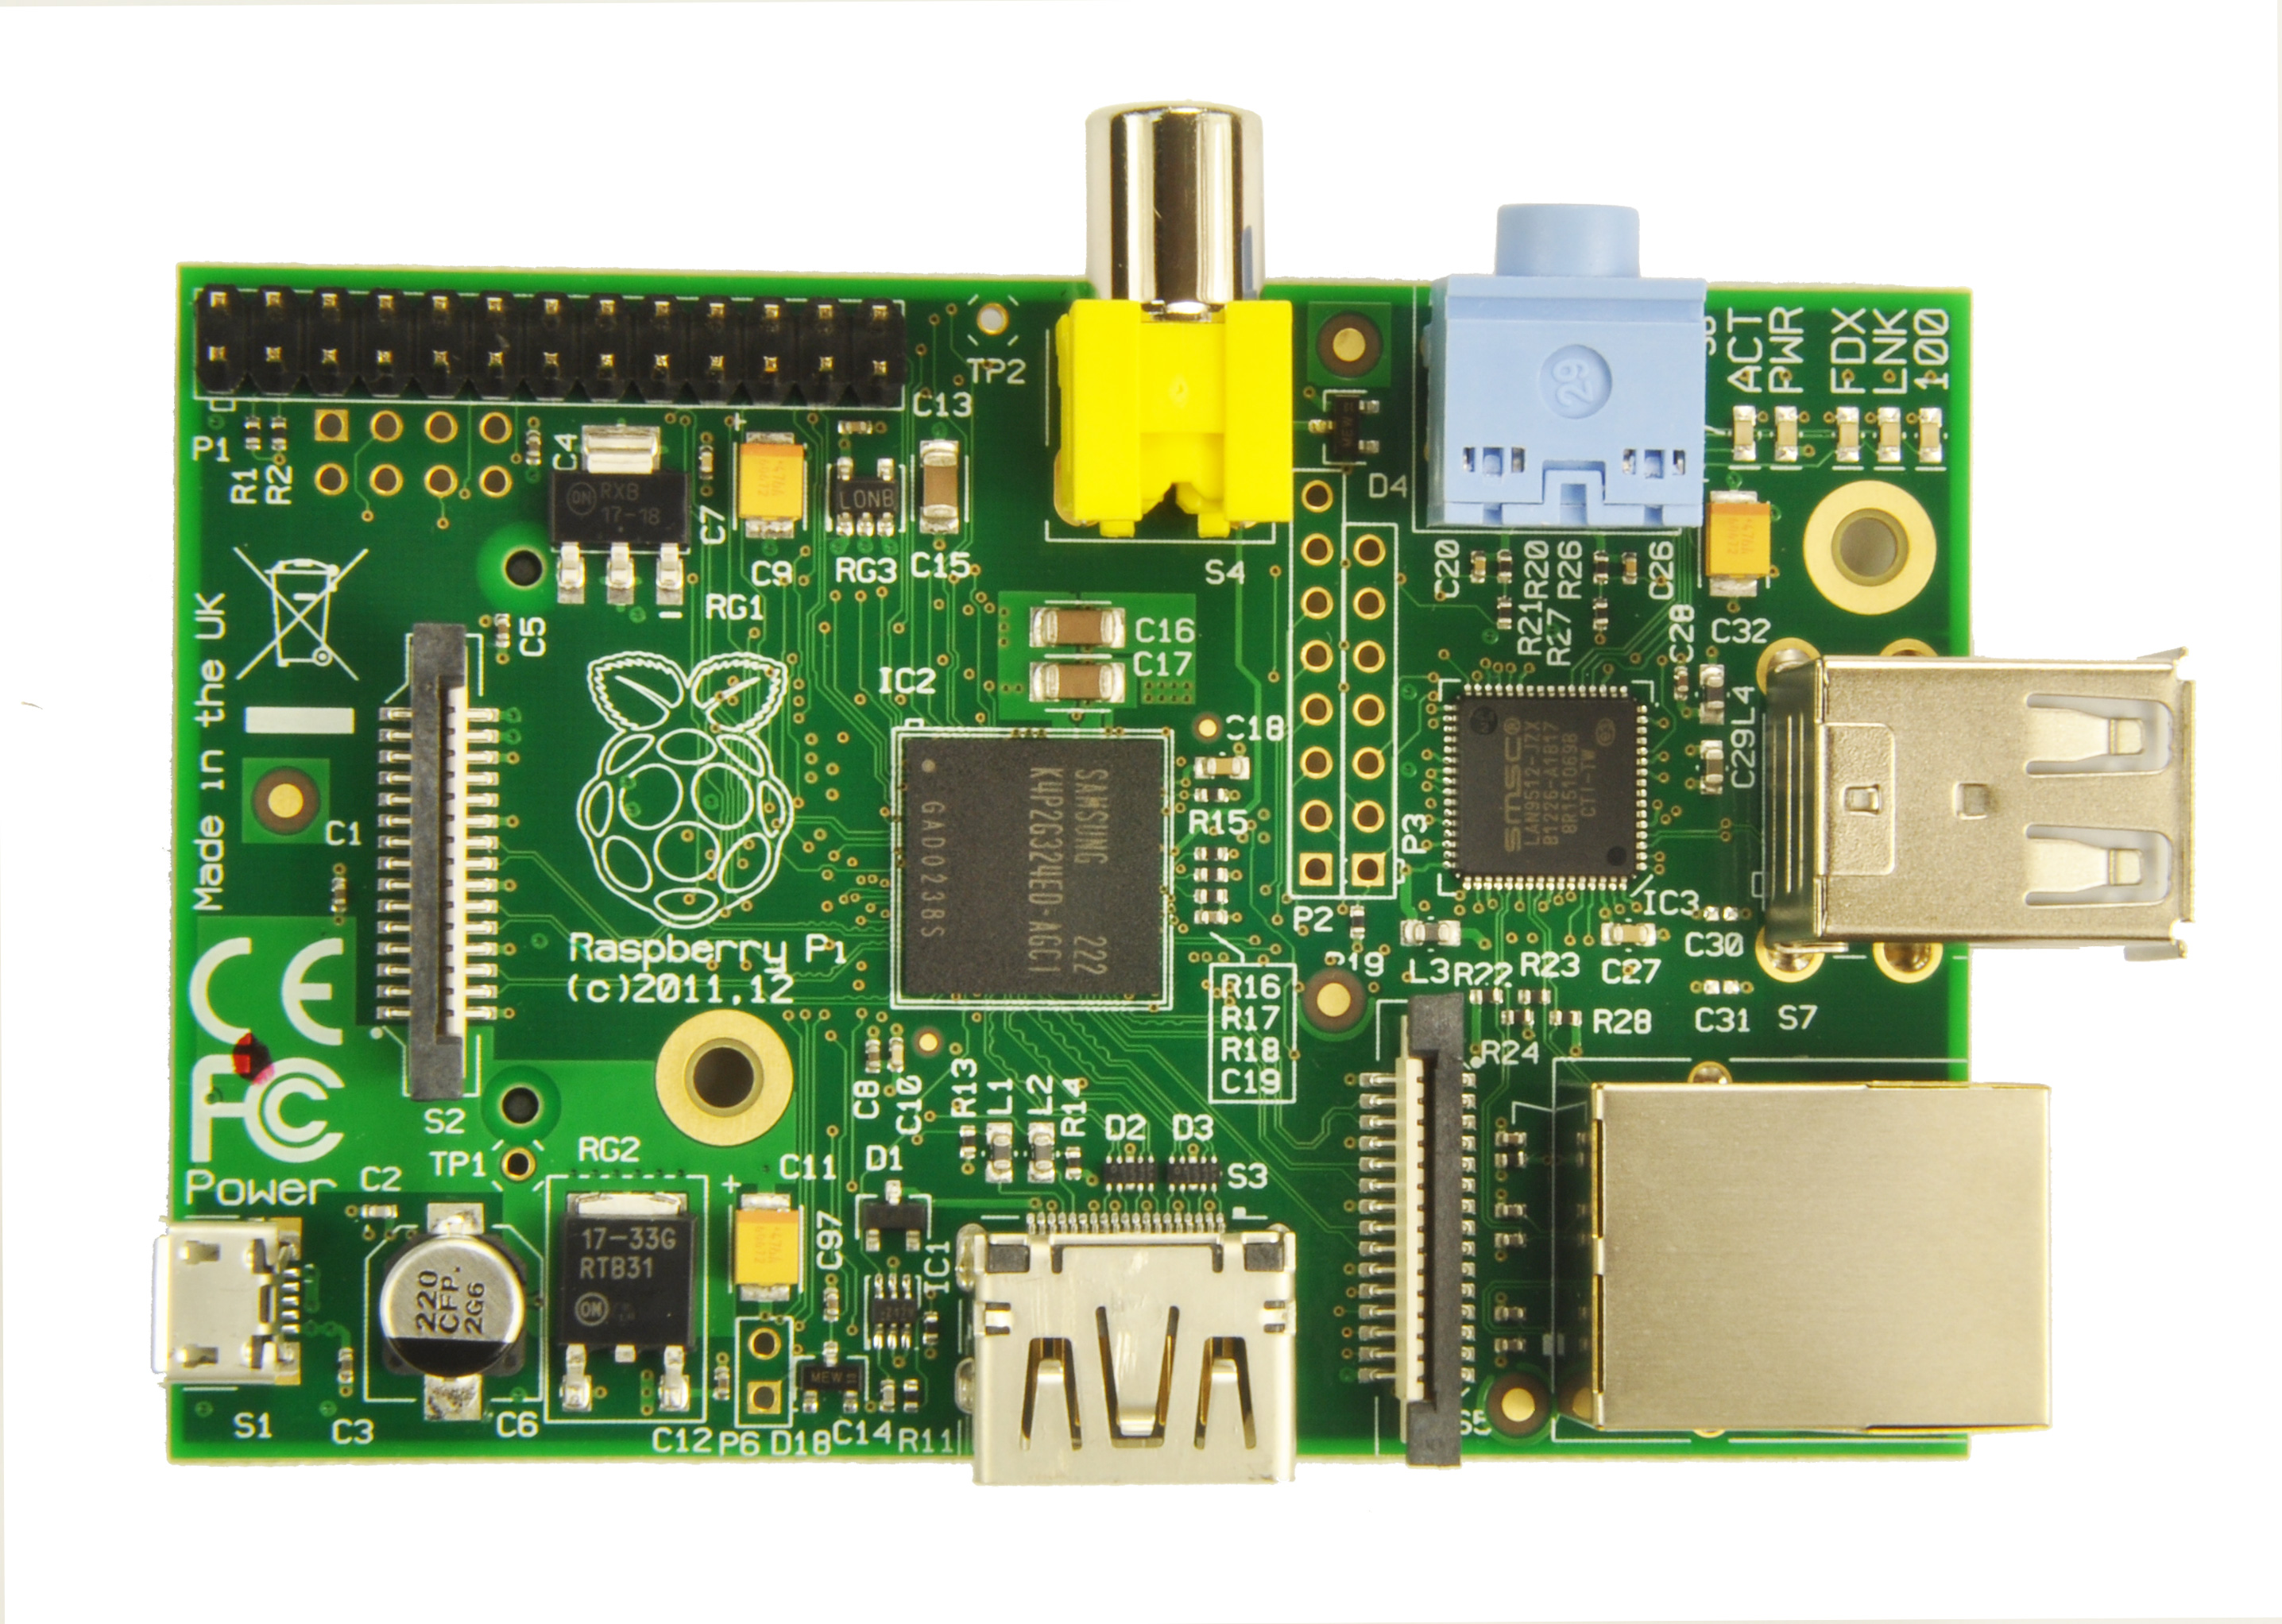
\includegraphics[width=0.5\textwidth]{RaspberryPi.jpg}
	\caption{\textit{RaspberryPi 1 Model B}}
	\label{fig:RaspberryPi}
\end{figure}
Šim \textit{RaspberryPi} modelim ir 512MB liela brīvpiekļuves atmiņa (RAM), 100mb tīkla ports, divi USB porti un \textit{Broadcom BCM2835} čips ar vienkodola \textit{ARM} tipa procesoru.

RaspberryPi ir arī aprīkots ar HDMI, audio izvades portiem, kā arī vispārēja lietojuma ievades un izvades adatām, padarot to par populāru rīku elektronikas un datoru entuziastu vidū, sniedzot teju neskaitāmus potenciālus pielietojumus.

\textit{BCM2835} čips izmanto \textit{ARM1176} procesoru, kurš ir sašaurinātas instrukcijkopas (angl. \textit{reduced instruction set computing} jeb \textit{RISC}) procesors, kas it īpaši ir populāri mobilajās ierīcēs. Sašaurinātā instrukcijkopa nozīmē, ka procesorus iespējams saražot ar mazāk tranzistoriem nekā ierastajiem sarežģītas instrukcijkopas procesoriem (angl. \textit{complex instruction set computing} jeb CISC), tādejādi samazinot procesoru ražošanas izmaksas, tā darbībā paterēto enerģiju un izvadīto karstumu.
Tipiski lietotājam tas nerada nekādu problēmu. Tomēr, RaspberryPi procesora arhitektūra ir būtiski atšķirīga no personālajos datoros ierastajiem CISC procesoriem, tāpēc liela daļa programmatūras nav oficiāli atbalstīta ar gataviem izpildfailiem un tie ir jākompilē, tādejādi palielinot sistēmas uzstādīšanas laiku.

\chapter{Drošība}

\section{Tipiskākie uzbrukumi un to novēršana} \label{Attacks}
\subsubsection{Uzbrukumi serverim}
Darba izstrādes gaitā tika uzstādīts \textit{RaspberryPi} un tas tika pievienots pie interneta. Tā kā izstrādes gaitā serveris nebija aiz ugunsmūra, tika novērots uzbrukuma mēģinājums atvērtajam \textit{SSH} (angl. \textit{Secure Shell}) portam, kas pēc noklusējuma ir 22. ports. Regulāri tika novēroti neizdevušies pieslēgšanās mēģinājumi \textit{root} kontam no nezināmas IP adreses, kas visticamāk bija pārlases uzbrukums (angl. \textit{brute-force attack}) parolei. Pēc darba vadītāja ieteikuma uz servera bija jau uzstādīta \textit{Fail2Ban} pretielaušanās sistēma, kas palīdz aizsargāties pret pārlases uzbrukumiem. Uz servera ir arī liegta iespēja pieslēgties ar \textit{root} kontu, izmantojot \textit{SSH}. Šādā veidā tika novērsts uzbrukuma mēģinājums serverim.

Tomēr jāpatur prātā, ka tiks veikti uzbrukumi atvērtajiem portiem, it īpaši noklusējuma \textit{SSH}, kā arī arī datubāzes portiem. Tāpēc ieteicams izmantot pretielaušanās programmatūru, kā arī nelielu papildus drošību iespējams iegūt, nomainot noklusējuma portus uz kādu neierastu portu.

\subsubsection{\textit{SQL} injekcija}
\textit{SQL} injekcija ir ļoti ierasts uzbrukums tīmekļa lietojumprogrammām. Bieži \textit{SQL} injekcijas mērķis ir apiet autorizācijas sistēmu, kā arī lasīt vai manipulēt datubāzes datus. To veic, manipulējot tīmekļa aplikācijai nosūtītos parametrus. Pieļaujot \textit{SQL} injekciju ir iespējams zaudēt visus datubāzē saglabātos datus, tāpēc jānodrošina, ka tā nav iespējama.

\textit{Rails} aplikācijās \textit{SQL} injekcija lielākoties nav problēma. Sekojot \textit{Rails} konvencijai ir grūti radīt \textit{SQL} injekcijas iespējas, tomēr ieteicams sekot \textit{Rails} pamācībā \cite{rails-guides} izteiktajiem padomiem. Tā kā \textit{SQL} injekcija ir ierasts un ļoti bīstams uzbrukums, tā iespējas meklē arī statiskās koda analīzes rīki. Izstrādes laikā vienā no iesūtījumiem \textit{VCS} tika atklāta un izlabota iespējama \textit{SQL} injekcijas vieta, izmantojot \ref{Testing} nodaļā aprakstīto \textit{Codacy} servisu.

\subsubsection{Starpvietņu skriptēšana}
Starpvietņu skriptēšana (angl. \textit{Cross Site scripting}) arī ir nopietns drošības risks. Praktiski visas vietas, kur lietotājs var ievadīt kādu informāciju, var radīt riskus drošībai. Uzbrucējam ir iespējams izmantot arī URL parametrus, lai izveidotu uzbrukumu. Izmantojot starpvietņu skriptēšanu, uzbrucējam var būt iespējams iegūt lietotāja sesijas datus.

Lai izvairītos no starpvietņu skriptēšanas, ir svarīgi filtrēt lietotāju ievadi, kā arī nodrošināt, ka, attēlojot ievadīto informāciju, tiek pieļauti tikai atbilstoši dati. Piemēram, nepieļaut \textit{HTML} \textit{<script>} tagus.
\textit{Rails} piedāvā vairākas palīgmetodes, kuras izmantojot iespējams izvairīties no starpvietņu skriptēšanas. Viena no tām ir \textit{sanitize()} metode, kuru var piemērot lietotāja ievades filtrēšanai. \textit{Rails} iesaka izmantot \textit{SafeErb} bibliotēku, kas atgādina par ievades filtrēšanu.

\section{Lietotāju autentiskums}
Sistēmai kopumā jāpārliecinās par trīs lietu autentiskumu:
\begin{itemize}
	\item mājaslapas lietotājs;
	\item karšu lasītājs;
	\item \textit{RFID} karte.
\end{itemize}
Lietotāji mājaslapā var ielogoties, izmantojot augstskolas piešķirto e-pasta adresi un pašu izvēlēto paroli. Lai nodrošinātu lietotāja autentiskumu, jānodrošina, ka lietotāja sesija netiek nolaupīta. Sesijas nolaupīšanu iespējams apgrūtināt, izmantojot \textit{HTTPS} savienojumu. \textit{HTTPS} nodrošina šifrētu savienojumu ar serveri, tādējādi būtiski palielinot drošību un apgrūtinot datu izgūšanu no pārtvertām tīkla paketēm, izmantojot kādu no pakešu analīzes rīkiem, piemēram, \textit{Wireshark} (\url{https://www.wireshark.org/}).

Tāpēc \textit{HTTPS} nodrošināšana ir viens no galvenajiem uzdevumiem. Tā uzstādīšanai nepieciešams iegūt uzticamu drošligzdu slāņa jeb {\textit{SSL} (angl. \textit{Secure Sockets Layer}) sertifikātu. Pastāv iespēja izveidot pašparakstītu sertifikātu, bet ikviens mūsdienīgs tīkla pārlūks par to brīdinās lietotāju, jo pastāv iespēja, ka sertifikāts nav autentisks. ir daudzas \textit{SSL} sertifikātu autoritātes, bet lielākā daļa no tām, kā \textit{IdenTrust} (\url{https://www.identrustssl.com/}) un \textit{DigiCert} (\url{https://www.digicert.com/}), ir komerciālas un par sertifikātiem ir jāmaksā. Viena no sertifikātu autoritātēm, kas tomēr piedāvā sertifikātus par brīvu, ir \textit{StartSSL} (\url{https://www.startssl.com/}). Tomēr sertifikāta iegūšana no \textit{StartSSL} var būt neskaidra un aizņemt daudz laika. Ir vēl viena jauna \textit{SSL} sertifikātu autoritāte \textit{Let's Encrypt} (\url{https://letsencrypt.org/}), kas piedāvā sertifikātus automatizētā veidā, ātri un par brīvu. Tāpēc tiks uzstādīts \textit{SSL} sertifikāts izmantojot \textit{Let's Encrypt} servisu.

Karšu lasītājs strādās līdzīgā veidā kā mājaslapas lietotāji. Karšu lasītājs būs pieslēdzies serverim, sūtīs un saņems no aplikācijas nepieciešamos datus. Karšu lasītāju ir nolemts ar serveri savienot, izmantojot bezvadu tīklu, tādējādi radot risku, ka tīkla paketes varētu tikt pārtvertas. Tomēr risks ir daudz mazāks, salīdzinot ar lietotājiem, jo serveris un karšu lasītājs atradīsies vienā telpā, tādējādi uzbrucējam jāatrodas sistēmas tuvumā, lai spētu pārtvert tīkla paketes no karšu lasītāja. Tomēr, lai novērstu pat tādu iespēju, līdzīgi kā ar lietotājiem, jānodrošina \textit{HTTPS} savienojums iepriekšapskatītajā veidā.
% Tā kā karšu lasītājs būs pievienots ar bezvadu tīklu, pastāv iespēja, ka kāds varētu karšu lasītāju imitēt. Lai apgrūtinātu uzbrukumu, ir iespējams karšu lasītāju saprogrammēt tā, lai tas veic vienkārsu datu šifrēšanu, pirms to izstūtīšanas.

\textit{RFID} kartes autentiskumu noteikt ir vissarežģītāk. Kaut arī \textit{RFID} kartēm ir unikāls kartes identifikators, nav pārliecības, ka pieejamais lasītājs to spēs nolasīt. Ir arī jāņem vērā, ka ir pieejami daudzi karšu lasītāji un arī rakstītāji. Uzbrucējs varētu nolasīt autorizētu karti un ierakstīt tās datus jaunā kartē. Visticamāk arī identifikatoru ir iespējams manipulēt, un to izmantot piekļūšanai telpā.
Tāpēc izstrādātā sistēma ļaus lietotājiem atcelt savas \textit{RFID} kartes piekļuvi telpai, tādējādi parūpējoties, ka karte nevar tikt izmantota piekļuvei, piemēram, tās nozaudēšanas gadījumā. Izstrādātā sistēma arī veiks momentuzņēmumus, kamēr telpas durvis būs atvērtas, ļaujot atklāt neautorizētas piekļuves gadījumus.

\section{RFID sistēmas}
